\documentclass[../notesdecours.tex]{subfiles}

\begin{document}
\part{Applications de la Mécanique Quantique}
\section{Interféromètre de Mech-Zehnder}
Cet exemple est tiré de l'optique. Nous allons regarder ce qu'il se passe en optique classique, et nous allons ensuite utiliser le formalisme quantique. Ce faisant, nous pourrons mettre en évidence les différences entre les deux. \\

\begin{center}
\begin{figure}[h]
\centering
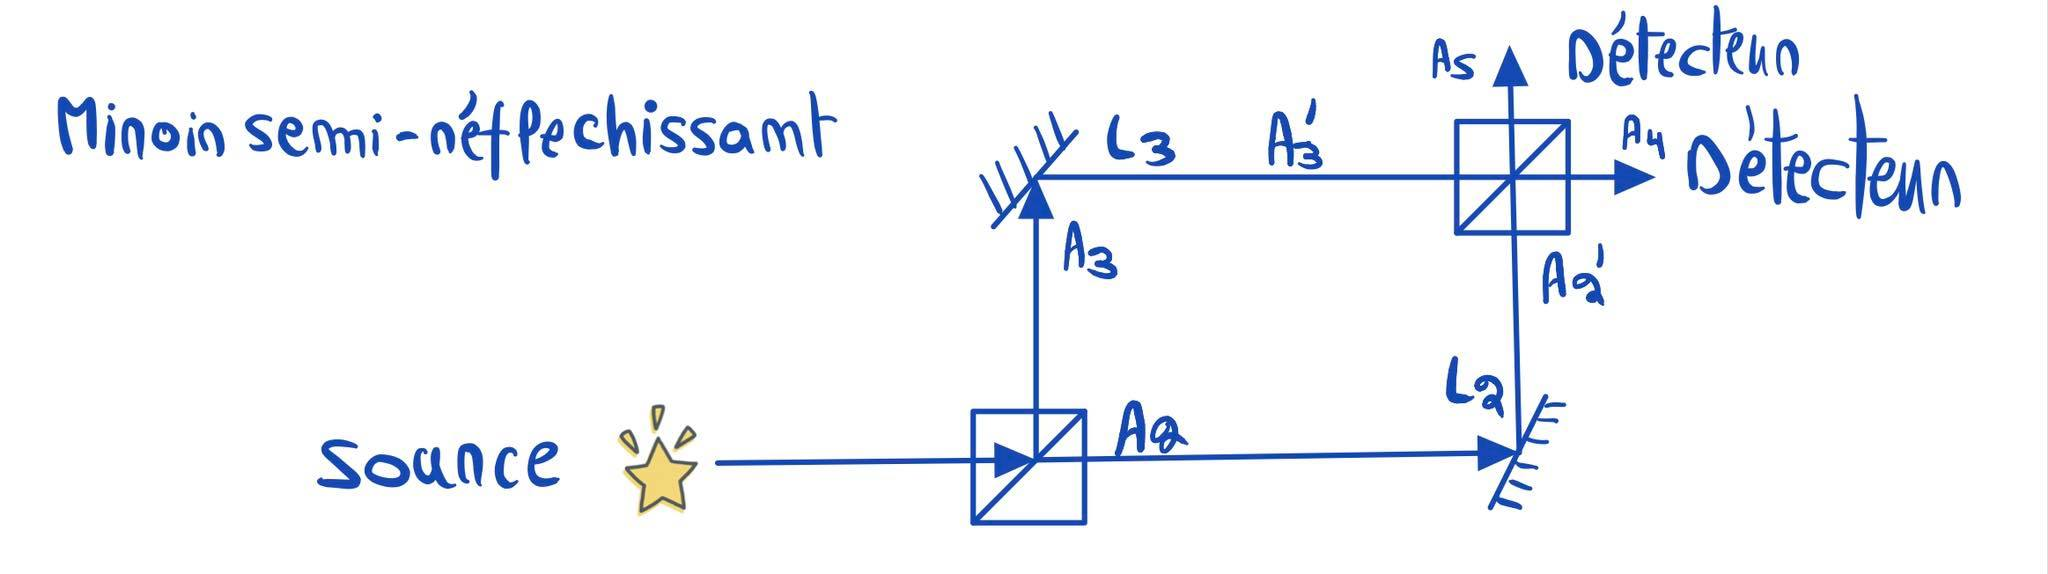
\includegraphics[width=0.80\textwidth]{Mach-Zehnder.png}
\caption{Représentation du principe de l'interféromètre de Mach-Zehnder. Notons que les longueurs $L_i$ représentent la longueur totale du trajet dans le chemin $i$ suivit.}
\end{figure}
\end{center}

\subsection{Lumière classique}
Au niveau des détecteurs, plusieurs chemins sont possibles, comme l'illustre l'image ci-contre.
\begin{center}
\begin{figure}[h]
\centering
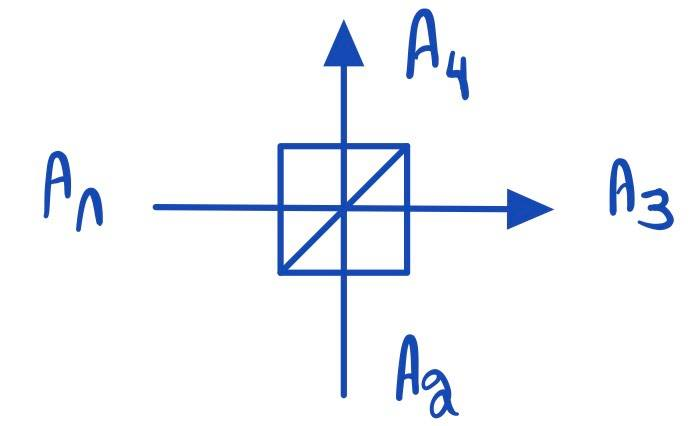
\includegraphics[width=0.50\textwidth]{bean.png}
\caption{Les ondes incidentes - arrivants de deux endroits différents, respectivement $A_1$ et $A_2$ peuvent suivre deux chemins différents : $A_3$ et $A_4$.}
\label{Interferometre}
\end{figure}
\end{center}
En supposant partant de la description d'une onde plane, nous pouvons écrire
\begin{subequations}
\begin{equation}
A_1 (t) = A_1e^{-i\omega t},
\end{equation}
\begin{equation}
A_2 (t) = A_2e^{-i\omega t},
\end{equation}
\end{subequations}
pour les ondes incidentes, ainsi que
\begin{subequations}
\begin{equation}
A_3 (t) = \cos\theta A_1e^{-i\omega t} + i \sin\theta A_2e^{-i\omega t}
\end{equation}
\begin{equation}
A_4 (t) = \cos\theta A_2e^{-i\omega t} + i\sin\theta  A_1e^{-i\omega t}
\end{equation}
\end{subequations}
pour les ondes sortantes.
\begin{remark} Par convention, les ondes transmises ne subissent aucun déphasage, là où les ondes réfléchies bénéficient d'un déphasage de $\pi / 2$. D'autres conventions sont possibles.\end{remark}

Notons que nous pouvons introduire un facteur $e^{ikL}$ tenant compte de la distance parcourue, i.e. un point en $x = 0$ peut-être décrit par $A(t) = Ae^{-i\omega t}$ et un point en $x = L$ peut-être décrit par $A'(t) = Ae^{-i\omega t}e^{ikL}$. Le détecteur est de sorte que $I(t) = e\norm{A(t)}^2$. Soit 
\begin{align*}
A(t) &= Ae^{-i\omega t}	&I_{Initial} = \norm{A(t)}^2
\end{align*}
Nous avons alors que
\begin{align*}
A_2 (t) &= \frac{A(t)}{\sqrt{2}}	&A_3 (t) = i\frac{A(t)}{\sqrt{2}}
\end{align*}
En particulier, nous pouvons écrire les chemins $A_2'$ et $A_3'$ de $\ref{Interferometre}$ selon
\begin{subequations}
\begin{equation}
A'_2 (t) = A_2 (t)e^{ikL_2}
\end{equation}
\begin{equation}
A'_3 = A_3 (t)e^{ikL_3}
\end{equation}
\begin{equation}
A_4 (t) = \frac{A'_3 (t)}{\sqrt{2}} + i \frac{A'_2 (t)}{\sqrt{2}} = \frac{A_3 (t)e^{ikL_3}}{\sqrt{2}} + i \frac{A_2 (t)e^{ikL_2}}{\sqrt{2}} = i\frac{A}{2} (e^{ikL_3} + e^{ikL_2})
\end{equation}
\begin{equation}
A_5 (t) = \frac{A'_2 (t)}{\sqrt{2}} + i\frac{A'_3 (t)}{\sqrt{2}} = \frac{A_2 (t)e^{ikL_2}}{\sqrt{2}} + i\frac{A_3 (t)e^{ikL_3}}{\sqrt{i}} = i\frac{A}{2} (-e^{ikL_3} + e^{ikL_2})
\end{equation}
\end{subequations}
En introduisant le terme $\Delta \Phi = kL_3 - kL_2$, nous pouvons conclure que
\begin{subequations}

\end{subequations}
\subsection{Lumière quantique}
{\color{red}{La ligne d'au-dessus est à compléter}}
L'algèbre est la même: l'interprétation change. 

\section{Oscillations de neutrinos}
Les neutrinons sont des particules neutres, intéragissant très faiblement avec la matière. Elle fût prédite par Pauli pour expliquer le spectre des $e^-$ dans la désintégration du $\beta : n \Rightarrow p^+ + e^- + \nu$.

\section{MASER $NH_3$}
Dans cette section, nous allons discuter d'un appareil fort pratique: le MASER\footnote{Acronyme anglais pour 'Microwave Amplicifaction by Stimulated Emission of Radiation'.} d'ammonium $NH_3$ ; l'un des ancêtres des LASER\footnote{Acronyme anglais pour 'Light Amplification by Stimulated Emission of Radiation'.}

\section{Spin $\frac{1}{2}$}
Nous voyons en cette section une très brève introduction à la quantification du moment angulaire en Mécanique Quantique. Pour ce faire, introduisons le $\mathcal{G}$roupe des $\mathcal{R}$otations.

Considérons l'ensemble des matrices $R \in \mathbb{R}^{3\times 3}$ telle que $R^TR = \mathbb{I}$. Si $\bm{n}$ est un vecteur unitaire de $\mathbb{R}^3$ et $\theta$ un angle, alors $R(\theta,\bm{n}$) est la rotation (en son sens anti-horlogique) autour de l'axe $\bm{n}$ d'angle $\theta$.
\begin{align*}
R(\theta,x) &= \begin{pmatrix}
1 & 0 & 0\\
0 & \cos\theta & -\sin\theta\\
0 & \sin\theta & \cos\theta
\end{pmatrix} = \exp (i\theta L_x)			&L_x = \begin{pmatrix}
0 & 0 & 0\\
0 & 0 & i\\
0 & -i & 0
\end{pmatrix}\\
R(\theta,y) &= \begin{pmatrix}
\cos\theta & 0 & \sin\theta\\
0 & 1 & 0\\
-\sin\theta & 0 & \cos\theta\\
\end{pmatrix} = \exp(i\theta L_y)		&L_y = \begin{pmatrix}
0 & 0 & -i\\
0 & 0 & 0\\
i & 0 & 0
\end{pmatrix}\\
R(\theta,z) &= \begin{pmatrix}
\cos\theta & -\sin\theta & 0\\
\sin\theta & \cos\theta & 0\\
0 & 0 & 1
\end{pmatrix} = \exp(i\theta L_z)		&L_z = \begin{pmatrix}
0 & i & 0\\
-i & 0 & 0\\
0 & 0 & 0
\end{pmatrix}
\end{align*}
Nous avons alors que $R(\theta,\bm{n}) = \exp (i\theta\bm{n}\cdot\bm{L})$, où $\bm{n}\cdot\bm{L} = n_iL_i$. Les vecteurs $L_x,L_y,L_z$ sont appelés les \emph{générateurs du $\mathcal{G}$roupe des $\mathcal{R}$otations}.\\

En physique, de nombreux objets (et non pas seulement les vecteurs) sont invariants ou se transforment sous l'effet d'une rotation. Une autre représentation du $\mathcal{G}$roupe des $\mathcal{R}$otations est l'ensemble des 3 opérateurs $J_x,J_y,J_z$ tels que $[J_x,J_y] = J_z$ (ainsi que toute permutation cyclique de cela) et tel que, sous toute rotation d'angle $\theta$ autour de $\bm{n}$, un état $\ket{\Psi}$ se transforme en
\begin{equation}
\ket{\Psi} \rightarrow \exp(i\theta\bm{n}\cdot\bm{J})\ket{\Psi}
\end{equation}

\begin{exemple}Les opérateurs
\begin{itemize}
\item $J_x = yp_z - zp_y$
\item $J_y = zp_x - xp_z$
\item $J_z = xp_y - yp_x$
sont des exemples de représentation du $\mathcal{G}$roupe des $\mathcal{R}$otations.
\end{itemize}
\end{exemple}
Un système est invariant par rotation lorsque
\begin{align*}
\exp (-itH) \exp (i\theta \bm{n}\cdot\bm{J})\ket{\Psi} &= \exp (i\theta \bm{n}\cdot\bm{J})\exp (-itH) \ket{\Psi}			&\forall \ket{\Psi},\forall \bm{n},\theta,t
\end{align*}
Cela revient à dire que \emph{faire une rotation} et ensuite \emph{évoluer dans le temps} est identique à \emph{évoluer dans le temps} et puis \emph{faire une rotation}.\\
\begin{lemma} Pour $\theta$ et $t$ infinitésimaux, nous avons que 
\begin{equation}
[H,J_x] = [H,J_y] = [H,J_z] = 0
\end{equation}
\end{lemma}
Les conséquences en sont nombreuses. Nous avons notamment alors que:
\begin{enumerate}
\item Si $\ket{\Psi(t)}$ est une solution de l'équation de Schrödinger \eqref{Postulat 4}, alors $\braket{\Psi(t)|J_x|\Psi(t)} = \braket{\Psi(0)|J_x|\Psi(0)}$.
\item Si $<ket{\Psi}$ est un vecteur propre de $J_x$,
\begin{equation}
J_x\ket{\Psi} = j\ket{\Psi}
\end{equation}
alors $\ket{\Psi(t)} = \exp (-iHt)\ket{\Psi}$ est aussi un vecteur propre de $J_x$.
\end{enumerate}
Le $\mathfrak{T}$héorème d'$\mathfrak{E}$mmy $\mathfrak{N}$öther nous apprend que la grandeur conservée par la symmétrie de rotation est le moment angulaire.

\subsection{Quantification du moment angulaire}
\begin{theorem}
Soit $[J_x,J_y] = iJ_z$. Nous avons alors que les valeurs propres de $J_z$ est un demi-entier: $0,\frac{1}{2}, 1, \frac{3}{2}, ...$.
\begin{equation*}
J_z \ket{\Psi} = m\ket{\Psi}
\end{equation*}
\end{theorem}
\begin{theorem}
Il existe une représentation non triviale du $\mathfrak{G}$roupe des $\mathfrak{R}$otations par des matrices $d\times d$. Dans ce cas, $J_z = -\frac{d}{2}, -\frac{d}{2}+1,...,+\frac{d}{2}$.
\end{theorem}
\begin{exemple}
Le cas le plus simple est celle des matrices de Pauline (matrices $2\times 2$):
\begin{center}
\begin{tabular}{c|c|c}
$\sigma_x = \begin{pmatrix}
0 & 1\\
1 & 0
\end{pmatrix}$ & $\sigma_x = \begin{pmatrix}
0 & -i\\
i & 0
\end{pmatrix}$ & $\sigma_x = \begin{pmatrix}
1 & 0\\
0 & -1
\end{pmatrix}$\\
$J_x = \frac{1}{2}\sigma_x$ & $J_y = \frac{1}{2}\sigma_y$ & $J_z = \frac{1}{2}\sigma_z$
\end{tabular}
\end{center}
Nous pouvons vérifier que les différentes relations démontrées ci-dessus sont respectées (exercice).
\end{exemple}
\end{document}